\chapter{Implementation}
In computergraphics, we are interested in synthesizing 2d images from a given scene containing our 3d geometries by using so called shader programs. This process is denoted as rendering.
The purpose of shader programs, which are executed directly on the GPU hardware device, is to compute the colorization and illumination of the objects living in our scene. All these computations happen in several stages and depend on the provided scene-input parameters like the camera, light sources, objects material constants and the desired rendering effect one is interested in to model. The shader stages are implemented sequencially as small little programs, the so called vertex-, geometry- and fragment-shaders. Those stages are applied within the rendering pipeline sequencially. 

Our shaders which we use are written in a high-level language called GLSL, the OpengGL Shading Language. The decission for using OpenGL has been made since my underlying framework, which is responsible for the precomputation of all scene date, is based on another framework, written in Java using JOGL in oder to communicate with the GPU and is also responsible to precompute all the relevant scene data. This framework, the so called jrtr framework, has been developed as an exercise during the class computer graphics held by M. Zwicker which I attended in autumn 2012. The framework itself has been used and further extended during this thesis quite a lot. All necessary input data required for our java framework in order to perform the shading is precomputed by using Matlab. This is basically addressing all the required precomputations for the provided heigh-fields, refering to computation of the inverse two dimensional Fourier transformations which are further explained within this chapter. The Matlab scripts themself rely on the provided snake nano-scaled sheds images, taken by AFM.

It's noteworthy that all the vertices are processed within the vertex-shader, whereas the fragement shader's responsibility is to perfrom pixelwise rendering, using the input from the vertex shader. Just remember, fragements are determined by a triple of vertices. hence each pixel has assigned a trilinear interpolated value of all input parameters of its spanning vertices.
Usually, all necessary transformations are applied vertex-wise, considering the vertex-shader as the precomputation stage for the later rendering within the rendering pipeline, in the fragment-shader. In the geometry shader, new vertices around a considered vertex can be created. this is useful for debugging - displaying normals graphically for example.

In this part of thesis we are going to explain how we render our BRDF formulation derived in the last section in practice. all the necessary computations in order to simulate the effect of diffraction are performed within a fragment shader. This implies that we are modeling the effect of diffraction pixelwise and hence the overall modeling quality and computional pace depends on rendering window's resolution.

By the end of this chapter we will have seen how our how our render works, what we have to precompute and how our shaders work. 


\section{Precomputations in Matlab}
Our first task is to precompute the inverse two dimensional discrete Fourier Transformations of a given snake shed patch of interest taken by AFM. For that purpose we have written a small Matlab script which offers a huge collection of mathematically, nummerically fast and stable algorithms. Our Matlab script reads a given image, which is representing a nano-scaled heightfield, and computes its inverse two dimensional DFT by using Matlab's internel inverse fast Fourier Transformation function, denoted by $ifft2$. Note that we only require once color channel of the input image since the input image is representing an heightfield, encoded by just one color. Basically, we are interested in computing the $ifft2$ for different powers of the input image since our taylor series approximation for the overall computation relies on this. Keep in mind that taking the Fourier Transformation of an arbitrary function will result in a complex valued output which implies that we will get a complex value for each pixel of our input image. Therefore, for each input image we get as many output images, representing the two dimensional inverse Fourier Transformation, as the minimal amount of taylor terms required for a well-enough approximation. In order to store our output images, we have to use 2 color channels instead just one like it was for the given input image. As an optimization step, we do not directly store images, rather we output binary files which contain all RGB values for each pixel in a row first, column last format. This allows us to have much higher precision for the output values and also it does not waste any color channels. Note that we have scaled each pixel value in a range between 0 and 1. Therefore, we have to remember store four scaling factors for each output image as well, which are the real and imaginary minimum and maximum values. Later, using linear interpolation within the shader, we will get back the image's original values. 

\begin{algorithm}[H]
\caption{Precomputation: Fourier images}
\begin{lstlisting}
% maxH:    A floating-point number specifying 
%          the value of maximum height of the 
%          height-field in MICRONS, where the 
%          minimum-height is zero. 
%         
% dH:      A floating-point number specifying 
%          the resolution (pixel-size) of the 
%          'discrete' height-field in MICRONS. 
%          It must less than 0.1 MICRONS to 
%          ensure proper response for 
%          visible-range of light spectrum.
%
% termCnt: An integer specifying the number of 
%          Taylor series terms to use.

function []= ComputeFFTImages(maxH, dh, termCnt)
dH = dh*1E-6;
% load patch into patchImg
patchImg = patchImg.*maxH;
% perform imrotate(patchImg, angle)
for t = 0 : termCnt
  patchFFT = power(1j*patchImg, t);
  fftTerm{t+1} = fftshift(ifft2(patchFFT));
  
  imOut(:,:,1)  = real(fftTerm{t+1});
  imOut(:,:,2)  = imag(fftTerm{t+1});
  imOut(:,:,3)  = 0.5;
  
  % perform imrotate(imOut, -angle)
  % find real and imaginary extrema of 
  % write imOut, extrema, dH, into files.
end
\end{lstlisting}
\end{algorithm}

The command fftshift rearranges the output of the ifft2 by moving the zero frequency component to the centre of the image. This is useful for visualizing a Fourier Transform with zero frequency components in the middle of the spectrum.


\begin{figure}[H]
  \centering
  \subfigure[Blaze Patch]{
    
\includegraphics[scale=0.25]{implementation/hf/blaze/blazeBig.png}
    \label{fig:matlabBlazePatch}
  }
~
  \subfigure[Extrema Plot]{
    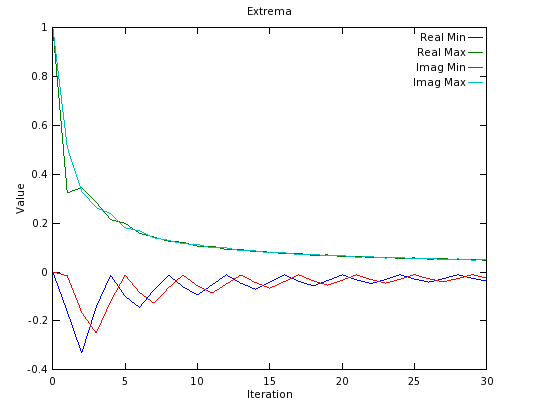
\includegraphics[scale=0.4]{implementation/hf/blaze/extrema.png}
    \label{fig:extremaBlaze}  
  }
  
  \subfigure[ImRe0]{
    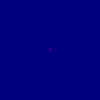
\includegraphics[scale=0.6]{implementation/hf/blaze/AmpReIm0.png}
    \label{fig:blazeftimre0}
  }
~
  \subfigure[ImRe1]{
    
\includegraphics[scale=0.6]{implementation/hf/blaze/AmpReIm1.png}
    \label{fig:blazeftimre1}
  }
~
  \subfigure[ImRe4]{
    
\includegraphics[scale=0.6]{implementation/hf/blaze/AmpReIm4.png}
    \label{fig:blazeftimre4}
  }
~
  \subfigure[ImRe10]{
    
\includegraphics[scale=0.6]{implementation/hf/blaze/AmpReIm10.png}
    \label{fig:blazeftimre10}
  }
~
  \subfigure[ImRe20]{
    
\includegraphics[scale=0.6]{implementation/hf/blaze/AmpReIm20.png}
    \label{fig:blazeftimre20}
  }
 
  
  \subfigure[Re0]{
    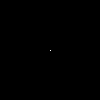
\includegraphics[scale=0.6]{implementation/hf/blaze/re0.png}
    \label{fig:blazeftre0}
  }
~
  \subfigure[Re1]{
    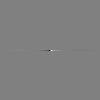
\includegraphics[scale=0.6]{implementation/hf/blaze/re1.png}
    \label{fig:blazeftre1}
  }
~
  \subfigure[Re4]{
    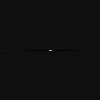
\includegraphics[scale=0.6]{implementation/hf/blaze/re4.png}
    \label{fig:blazeftre4}
  }
~
  \subfigure[Re10]{
    
\includegraphics[scale=0.6]{implementation/hf/blaze/re10.png}
    \label{fig:blazeftre10}
  }
~
  \subfigure[Re20]{
    
\includegraphics[scale=0.6]{implementation/hf/blaze/re20.png}
    \label{fig:blazeftre20}
  }
  
  \subfigure[Im0]{
    
\includegraphics[scale=0.45]{implementation/hf/blaze/im0.png}
    \label{fig:blazeftim0}
  }
~
  \subfigure[Im1]{
    
\includegraphics[scale=0.6]{implementation/hf/blaze/im1.png}
    \label{fig:blazeftim1}
  }
~
  \subfigure[Im4]{
    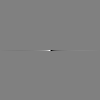
\includegraphics[scale=0.6]{implementation/hf/blaze/im4.png}
    \label{fig:blazeftim4}
  }
~
  \subfigure[Im10]{
    
\includegraphics[scale=0.6]{implementation/hf/blaze/im10.png}
    \label{fig:blazeftim10}
  }
~
  \subfigure[Im20]{
    
\includegraphics[scale=0.6]{implementation/hf/blaze/im20.png}
    \label{fig:blazeftim20}
  }
  
  \label{matlabBlazeFourierImages}
  \caption{Blaze}
\end{figure}


TODO: say something about output?

\section{Our Java Renderer}
In autumn 2012, during the semester I have attented the class computer graphics held by M. Zwicker. During the whole class we have developed a so called real time renderer program written in java as a series of homework assignments in order to be admitted to the final exam. The architecture of the program is divided into two parts: a rendering engine, the so called jrtr (java real time renderer) and an application program, denoted as scene.

\begin{figure}[H]
  \centering
  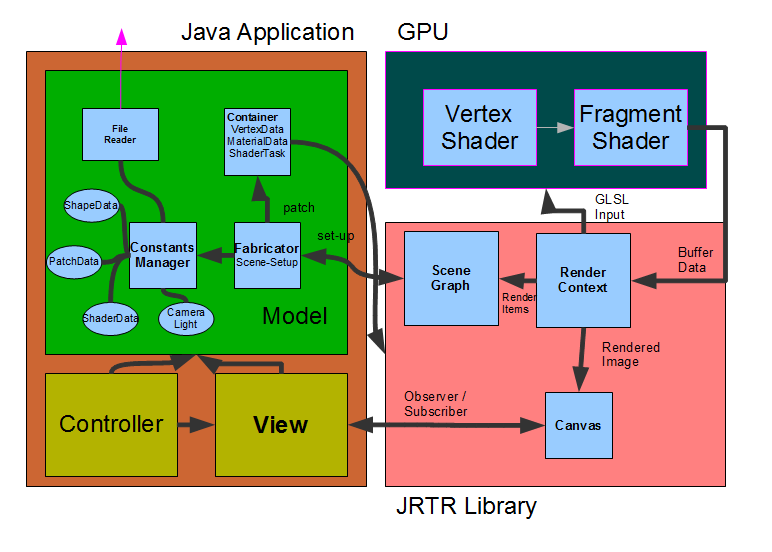
\includegraphics[scale=0.7]{implementation/framework.png}
  \label{rendererArchitecture}
  \caption{Renderer Architecture}
\end{figure}

the scene application program task was basically to define the whole scene we is going to be rendered within jrtr later.
A scene consists of the setup of the world camera, definitions of light source, frustum, geometries which live in our scene and their material constants. Such materials are textures for example. All those scene attributes are managed within jrtr. In the application program, there only happens their definition.
The minimal definition of a geometry is given by its wireframe mesh. This is a datastructures consisting of vertices each stored as a triple of xyz positions in an float array and triangles each defined by a triple of vertex-indices which form a fragment each stored in an integer array. It is possible to assing additional geoemtry data like a color for each vertex, normals and texture coordinates.
All whole scene is stored within container data-structures, defined and managed within jrtr, like a scene graph, which contains all geometries and their transformations in a tree like structured hierarchy. The geometries themself are stored within an container, containing all vertex attributes and the material constants.
The jrtr rendering engine uses a low-level API, called openGL in order to communicate with the grpahcis processor unit (GPU). Within jrtr, the whole resource-management for the rendering pipeline place, i.e. all required low-level buffers are allocated, flushed and assigned by the scene data attributes. jrtr also offers also the possibility to assign arbitrary shaders.
   
\subsection{Scene}
what is done here 
reworked such that it is mvc-architecute based
user-interaction: handlers in GUI.
which geometries are defined
what material constants are defined: mention fabricators: light, camera, materials,...
file readers: monkey

\subsection{jrtr Framework}
shader tasks
assign all shader inputs: like t0 and so on
load fourier images and assign to buffers
snapshot functionality
shaders: diffraction shader


\section{GLSL Diffraction Shader}
TODO: start using the final findings from chapter 2 and substitute

\subsection{Vertex Shader}
The first computional stage within our rendering pipeline is computing all necessary per vertex data. Those computations are preformed in the vertex shader. In our case, we compute for any vertex of our current geometry the direction vectors $k1$ and $k2$ described like previousely in the tangent space. Initially all input data lives in its own space. Hence, we first have to transfrom all input data into the same space in order to use it for later computations within the fragment shader. We are going to transform k1 and k2 into the so called tangent space which. Furthermore, we have also to realign our local coordinate system. This is why there is an rodrigues rotation also involved. In order to avoid scaling issues and since we are only interested in the direction of the vectors k1 and k2, we have to normalize them, too. Last, we also output the position of the current vertex transfomed into the projective camera space.
  
explain $cop_w$
modelM
other shader assigned inputs

\begin{algorithm}[H]
  \caption{Vertex diffraction shader}
  \begin{algorithmic}
    \ForAll{$Vertex \thinspace v \in Shape$}
      \State $ vec3 N = normalize(modelM * vec4(normal,0.0)).xyz$
      \State $ vec3 T = normalize(modelM * vec4(tangent,0.0)).xyz$
      \State $ T = rotateRodrigues(T, N, phi)$
      \State $ vec3 B = normalize(cross(N, T))$
      \State $ vec3 Pos = ((cop_w-position)).xyz$
      \State $ vec4 lightDir = (directionArray[0])$
      \State $ lightDir = normalize(lightDir)$
      \State $ l = projectVectorOnTo(lightDir, TangentSpace)$
      \State $ p = projectVectorOnTo(Pos, TangentSpace)$
      \State $normalize(l); normalize(p)$
      \State $gl_Position = projection * modelview * position$
    \EndFor
  \end{algorithmic}
\end{algorithm}


\subsection{Fragment Shader}
The purpose of a fragment shader is to render per fragment. A fragment is spanned by three vertices of a given mesh. For each pixel within all the output from the vertex shaders of its corresponding vertices is then trilinearly interpolated, depending on the pixel's position within the fragment, and passed into its fragment shader program.
Furthermore, there can be additional input be assigned which is not directly interpolated from the output of vertex shader programs. Our fragment shader just relies on k1 and k2 from its vertex shaders for the computation of the effect of diffraction.
There are some values preliminarily assigned to our fragment shader during the opgenGL setup within our java program, like all references to the image buffers, containing the Fourier Transformations, the number of taylor step approximations, the minimal and maximal wavelength, other lookup values like the scaling factors, a reference to a lookup table containing the $CIE_{XYZ}$ color weights for our wavelength domain and other scaling constants.

Our shader performs an on-the-fly numerical integration for the integral in the derivation using trapeziodal rule with uniform discretization of the $\lambda$ dimension at a resolution of 5nm. To compute $F_{dtft}\{p\}$ terms the shader uses he precomputed DFTs for the Taylor series terms given in the derivation. The Gaussian window approach is performed for each discrete $\lambda$ value using a window large enough to span $4\sigma_f$ in both dimensions. For computing DFT tables we generally use nanostructure hieghtfields that span at least 65$\mu m^2$ and are sampled with resolution of at least 100nm. This ensures that the spectral response encompasses al the wavelengths in the visible spectrum, i.e. from 380nm to 780nm. Note that this shader is not very fast in hardly can be denoted being interactive. 

mention we uniform discretize $\lambda$ for a given (u,v) which implies compressing sampled frequencies to the region near to the origin (of their frequency domain). 
For natural structures in nano-scale, most of their spectral energy lies at lower spatial frequencies which maps closer to region $(u,v) = (0,0)$ than higher frequencies. This is why We have chosen to sample (u,v) space non-linearly. We use 30 Taylor-terms for our approximation approach which has an error below Y, proven in the previous derivation chapter.

\begin{algorithm}[H]
  \caption{Fragment diffraction shader}
  \begin{algorithmic}[1]
    \ForAll{$Pixel \thinspace p \in Fragment$}
      \State \init $BRDF_{XYZ}, BRDF_{RGB}$ \myto $vec4(0.0)$
      \State $(u,v,w) = \hat{\mathbf{k_1}}-\hat{\mathbf{k_2}}$
      \For{$(\lambda = \lambda_{min};\thinspace \lambda \leq \lambda_{max};\thinspace \lambda = \lambda + \lambda_{step})$}
        \State $xyzWeights = getClrMatchingFnWeights(\lambda)$
        \State $lookupCoord = getLookupCoord(u, v, \lambda)$
        \State \init $P$ \myto $vec2(0.0)$
        \State $k = \frac{2\pi}{\lambda}$
        \For{$(n = 0$ \myto $MAXTAYLORTERMS)$}
          \State $taylorScaleF = \frac{(kw)^n}{n!}$
          \State \init $F_{fft}$  \myto $vec2(0.0)$
          \State $anchorX = int(floor(center.x + lookupCoord.x * fftImWidth)$
          \State $anchorY = int(floor(center.y + lookupCoord.y * fftImHeight)$
          \For{$(i=(anchorX-winW)$ \myto $(anchorX + winW + 1))$}
            \For{$(j=(anchorY - winW)$ \myto $(anchorY + winW + 1))$}
              \State $dist = getDistVecFromOriginFor(i,j)$
              \State $position = getLocalLookUp(i,j,n)$
              \State $fftVal = getRescaledFourierTextureValueAt(position)$
              \State $fftVal \asteq getGaussWeightAtDistance(dist)$
              \State $F_{fft} \pluseq fftVal$
            \EndFor
          \EndFor
          \State $P \pluseq taylorScaleF*F_{fft}$
        \EndFor
        \State $xyzPixelColor \pluseq dot(vec3(\left|P\right|^2), xyzWeights)$
      \EndFor
      \State $BRDF_{XYZ} = xyzPixelColor*C(\hat{\mathbf{k_1}},\hat{\mathbf{k_2}})*shadowF$
      \State $BRDF_{RGB}.xyz = D_{65}*M_{XYZ-RGB}*BRDF_{XYZ}.xyz$
      \State $BRDF_{RGB}= gammaCorrect(BRDF_{RGB})$
    \EndFor
  \end{algorithmic}
\end{algorithm}


\myparagraph{From line 4 to 26:} 
Within this loop happens the uniform sampling along lambda space. At line 5: $getClrMatchingFnWeights(\lambda)$ computes the color weights for the current wavelength by bilinear interpolation from the two closest given $CIE_{XYZ}$ color weights for our current wavelength $\lambda$. At line 6: $getLookupCoord(u, v, \lambda)$ computes the current coordinate for the texture lookup in our precomputed ifft2 images. 

\myparagraph{From line 9 to 24:} 
Within this loop happens the taylor series approximation till a predefined upper bound, denoted as $MAXTAYLORTERMS$.
Basically, the spectral response is approximated for our current $(u,v,\lambda)$. Furthermore, neighborhood-bounds for the upcoming gaussian windowing-sampling-approach are computed, denoted as anchorX and anchorY.

\myparagraph{From line 14 to 22:} 
In this most inner loop the convolution of the gaussian window with the inverse FFT of the patch is pixelwise performed. 
$getGaussWeightAtDistance(dist)$ computes $~\eqref{eq:gaussweight}$ from the distance between the center of the FFT image with the current position in the neighborhood in texture space. $getRescaledFourierTextureValueAt(position)$ rescales the current computed value by the precomputed extrema values since all image values are scaled between 0 and 1. At line 27 $C(\hat{\mathbf{k_1}},\hat{\mathbf{k_2}})$ is multiplied in front of the current computed pixel-color. This terms was introduced in the derivation chapter and is the product of equation $~\eqref{eq:cfact}$

The $C$ term includes is the gain factor $\ref{eq:cfact}$. We compute this by using the so called Schlick approximation $\ref{eq:schlickapprox}$ using an reactive index at 1.5 since this is close to the measured value from snake sheds.

Our BRDF values are scaled by s shadowing function as described in (SEE REFERENCES - PAPER), since most of the grooves in the snake skin nano-structures would from a V-cavity along the plane for a wave front with their top-edges at almost the same height.   

\section{Technical details}
\myparagraph{Texture lookup}
In a GLSL shader the texture coordinates are normalized which means that the size of the texture maps to the coordinates on the range $[0,1]$ in each dimension. By convention the the bottom left corner of an image has the coordinates $(0,0)$, whereas the top right corner has the value $(1,1)$ assigned. 

Given a nano-scaled surface patch P with a resolution $A$ by $A$ microns stored as an $N$ by $N$ pixel image $I$.
Then one pixel in any direction corresponds to $dH = \frac{A}{N} \mu m$. 
In Matlab we compute a series of $n$ output images $\{I_{out_1},...,I_{out_n}\}$ from $I$, which we will use for the lookup in our shader. For the lookup we use scaled and shifted $(u,v)$ coordinates from $\ref{eq:uvw}$. 

Since the zero frequency component of output images was shifted towards the centre of each image, we have to shift $u$, $v$ to the center of the current $N$ by $N$ pixel image by a bias $b$. Mathematically, the bias is a constant value is computed the following:

\begin{align}
    b
    &= (N \% 2 == 0) \quad ? \quad \frac{N}{2} : \frac{N-1}{2}
\label{eq:bias}
\end{align}

For the scaling we have to think a little further: lets consider a $T$ periodic signal in time, i.e. $x(t) = x(t+nT)$ for any integer n. After applying the DFT, we have its discrete spectrum $X[n]$ with frequency interval $w0 = 2pi / T$ and time interval $t0$. Let $k = \frac{2 \pi}{\lambda}$ denote the wavenumber for the current wavelength $\lambda$.
Ehen the signal is both periodic with time period $T$ and discrete with time interval $t_0$ then its spectrum should be both discrete with frequency interval $w_0$ and periodic with frequency period $\Omega = \frac{2 \pi}{t_0}$. This gives us the idea how to discretize the spectrum: Let us consider our Patch $P$ assuming it is distributed as a periodic function on our surface. Then, its frequency interval along the x direction is $w_0 = \frac{2 \pi}{T} = \frac{2 \pi}{N*dH}$. 
Thus only wave numbers that are integer multiples of $w_0$ after a multiplication with $u$ must be considered, i.e. $ku$ is integer multiple of $w_0$. Hence the lookup for the u-direction will look like:

\begin{align}
    \frac{ku}{w_0} 
    &= \frac{ku N dH}{2 \pi} \\
    &= \frac{u N dH}{\lambda}
\label{eq:scalelook}
\end{align}

Using those findings $\ref{eq:bias}$, $\ref{eq:scalelook}$, the final $(u,v)$ texture lookup-coorinates for the current wavelength $\lambda$ in iteration, will then look like:

\begin{equation}
  (u_{lookup}, v_{lookup}) = \left( \frac{u N dH}{\lambda} + b, \frac{v N dH}{\lambda} + b \right)
\label{eq:ublookup}
\end{equation}  

Note for the windowing approach we are visiting a one pixel neighborhood for each pixel $p$. 
This is like a base change with $(u_{lookup}, v_{lookup})$ as new coordinate system origin. The lookup coordinates for the neighbor-pixel $(i,j)$ are:

\begin{equation}
  (u_{lookup}, v_{lookup}) = (i,j)-(u_{lookup}, v_{lookup})
\label{eq:gaussianwindow}
\end{equation}

\myparagraph{Space Transformations}
what spaces are involved.

\myparagraph{Texture Blending}
The final rendered color for each pixel is a weighted average of different color components, such as the diffraction color, the texture color and the diffuse color. In our shader the diffraction color is weighted by a constant $w_{diffuse}$. the texture color is once scales by a binary weight determined by the absolute value of the Fresnel Term $F$ and once by $1-w_{diffuse}$. 

\begin{algorithm}[H]
  \caption{Texture Blending}
  \begin{algorithmic}
    \State $\alpha = (abs(F) > 1) ? 1 : 0$
    \State $c_{out} =(1-w_{diffuse})*c_{diffraction} + (1-\alpha)*c_{texture} + w_{diffuse}*c_{texture})$
  \end{algorithmic}
\end{algorithm}

\myparagraph{Color Transformation}
mention CIE XYZ to CIE RGB, D65, gamma correction.

\section{Discussion}
Our Current approach will sample the whole wavelength spectrum for each pixel but there is an optimization possible:
Lets consider $(u,v,w)$ defined as $\ref{eq:uvw}$. Let $d$ be the spacing between two slits of a grating. For any $L(\lambda) \neq 0$ it follows $\lambda_{n}^{u} = \frac{d u}{n}$ and $\lambda_{n}^{v} = \frac{d u}{n}$. For $n = 0$ there it follows $(u,v)=(0,0)$. 
If $u,v > 0$
\begin{align*}
    N_{min}^{u} = \frac{d u}{\lambda_{max}} \leq n_{u} \leq \frac{d u}{\lambda_{min}} = N_{min}^{u}\\
    N_{min}^{v} = \frac{d v}{\lambda_{max}} \leq n_{v} \leq \frac{d v}{\lambda_{min}} = N_{min}^{v}
\end{align*}
If $u,v < 0$
\begin{align*}
    N_{min}^{u} = \frac{d u}{\lambda_{min}} \leq n_{u} \leq \frac{d u}{\lambda_{min}} = N_{max}^{u}\\
    N_{min}^{v} = \frac{d v}{\lambda_{min}} \leq n_{v} \leq \frac{d v}{\lambda_{min}} = N_{max}^{v}
\end{align*}

By transforming those equation to $(\lambda_{min}^{u}, \lambda_{min}^{u})$, $(\lambda_{min}^{v}, \lambda_{min}^{v})$ respectively for any $(u,v,w)$ for each pixel we can reduce the number of required iterations in our shader.

Note: issue at center, specularity handled seperately.
pq-apporach.
